% Ray Migneco

\documentclass[12pt]{article}
\usepackage{alltt,epsfig}
\usepackage{amsmath}
\usepackage{fancyhdr}
\usepackage{wrapfig}
\usepackage{setspace}
\usepackage{multirow}
\usepackage{multicol}

\marginparwidth 0pt
\oddsidemargin  0pt
\evensidemargin  0pt
\marginparsep 0pt

\topmargin   -0.5in
\textwidth   6.5in
\textheight  9 in

\pagestyle{fancy}

\fancyhead{}
\fancyfoot{}

\chead{Summer Music Technology 2013}
\lfoot{MET-lab}
\cfoot{\thepage}
\rfoot{Drexel University}

\renewcommand{\headrulewidth}{0pt}
\renewcommand{\footrulewidth}{0pt}

%\newcommand{\ben}{\begin{enumerate}}
%\newcommand{\een}{\end{enumerate}}

\begin{document}

% Make the document title
\begin{center}
{\Large \bf Acoustic Resonance Lab}\\
\end{center}

\vspace{0.2in}

%{\bf Instructor: Adam Berkowitz}

\vspace{.2in}

% Introduction
\section{Introduction}
This activity introduces several concepts that are fundamental to understanding how sound is produced in musical instruments. We'll be measuring audio produced from acoustic tubes.

\textbf{General Notes}

\begin{itemize}
\item Work in groups of 2 or 3 
\item Divide up the tasks amongst your group members so everyone contributes
\end{itemize}

\textbf{Equipment Check} Make sure you have the following:

\begin{multicols}{2}
\begin{itemize}
\item (2) iPads
\item (1) Tape Measure
\item (1) Amplifier
\item (1) iRig Pre-Amp
\item (1) XLR cable
\item (1) Microphone
\item (1) Adjustable PVC tube with speaker
\item (1) RCA to 1/8" audio cable
\item (2) Pieces of speaker wire
\item (1) Pair of Alligator clips
\end{itemize}
\end{multicols}
% 
% \begin{figure}[h]
% \centering
% \includegraphics[width= .4 \textwidth]{images/gettingstarted/MIAparts2.pdf}
% \caption{Required Equipment.}
% \label{components}
% \end{figure}
% 
% \newpage

\section{Sound Generation Setup}
We will use one iPad to generate tones that will play through our tube. However, the iPad can't provide enough power to drive the speaker, so we need to connect it to an amplifier. From here on, we'll refer to this iPad as the \emph{\textbf{Synthesizer}}.

\begin{enumerate}
\item Plug the Amplifier's power cord into an outlet. \textbf{DO NOT TURN IT ON}.
\item Plug one end of the 1/8" audio cable to the iPad's headphone output jack. Plug the other end into the Amplifier's \textbf{Input} jack.
\item Attach the alligator clips to the speaker wires on the Amplifier's \textbf{Output} jack. Attach the other end of the clips to the speaker terminals (the speaker should be mounted to the tube).
\end{enumerate}

\section{Sound Analysis Setup} 
In order to measure the audio, we need to record audio from a microphone. The other iPad will be used to record sound. We will refer to this iPad as the \emph{\textbf{Analyzer}}.

To set up the microphone on the \textbf{Analyzer} iPad, follow the directions below. See Fig. \ref{micSetup} for how to connect the cables.

\begin{enumerate}
 \item Plug the iRig Pre-Amp into the headphone jack of the \textbf{Analyzer}.
 \item Take the XLR cable and connect one end to the iRig and the other to the microphone.
 \item Turn the iRig on by setting it to \textbf{+48V}.
 
\end{enumerate} 

\begin{figure}[!h]
\centering
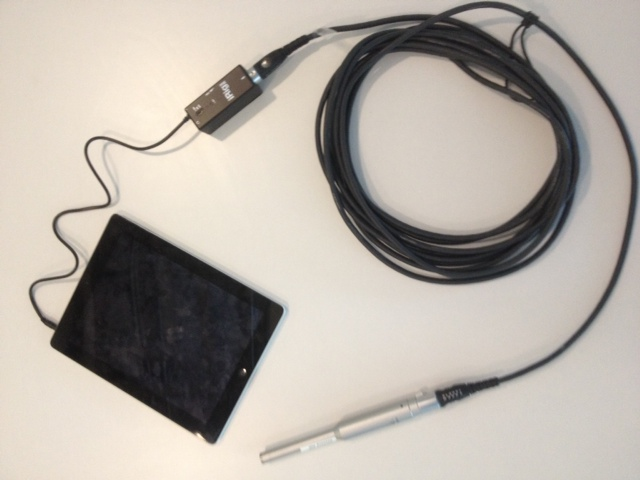
\includegraphics[width=4in]{images/gettingstarted/iRigSetup}
\caption{Microphone setup for an iPad}
\label{micSetup}
\end{figure}

Open the iPad application called SoundAnalysis on the \textbf{Analyzer} iPad. This application records sound input through the microphone and displays the soundwave's frequency spectrum.

\begin{figure}[!h]
\centering
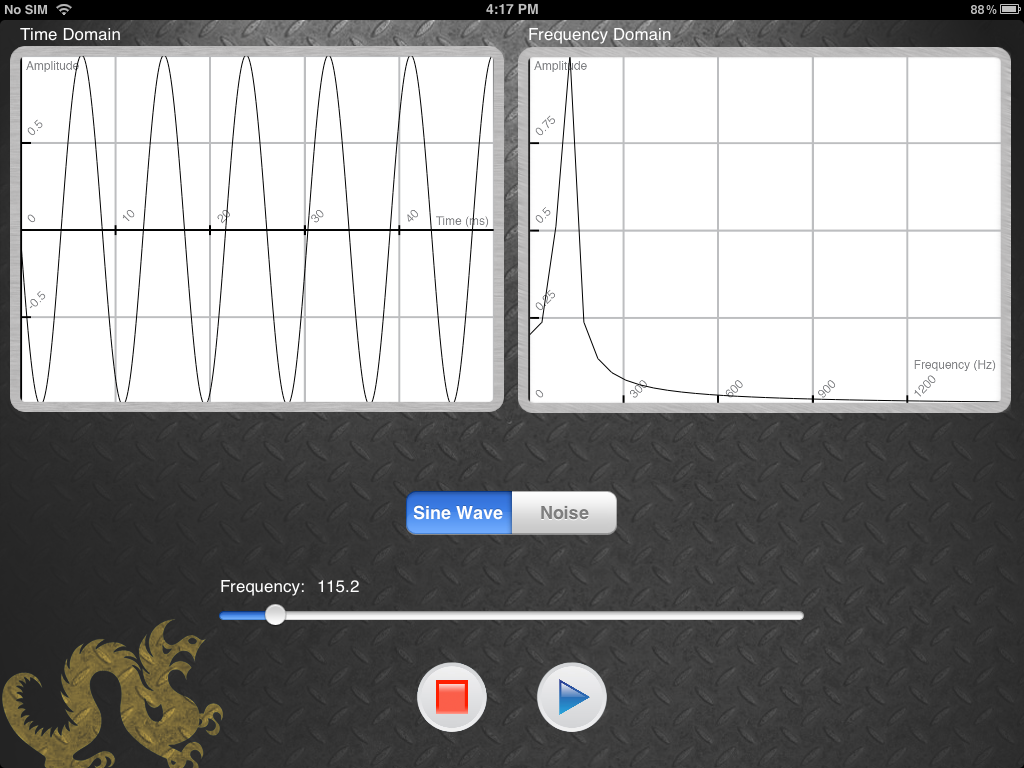
\includegraphics[width=6in]{images/Screenshots/SoundCannonApp.PNG}
\caption{Sound generation program for the synthesizer iPad. The left window displays the wave form and the right window displays the frequency spectrum.}
\label{synthesizerProgram}
\end{figure}

\section{Generating and Measuring Tones} 
We can now begin driving the tubes with various sound sources and measuring the output. The application SoundCannon allows us to generate a variety of sounds and tones. Using the \textbf{Synthesizer} iPad, do the following:

\begin{enumerate} 
\item Open the SoundCannon app on the \textbf{Synthesizer} iPad, it should look like Figure 2.
\item Make sure the Amplifier volume is set to a reasonable level and then turn it on.
\item Select the Sine Wave box and move the Frequency slider to change the pitch of tone.
\item Observe the Frequency Spectrum window (on the right) as you move the Frequency slider.

\begin{figure}[!h]
\centering
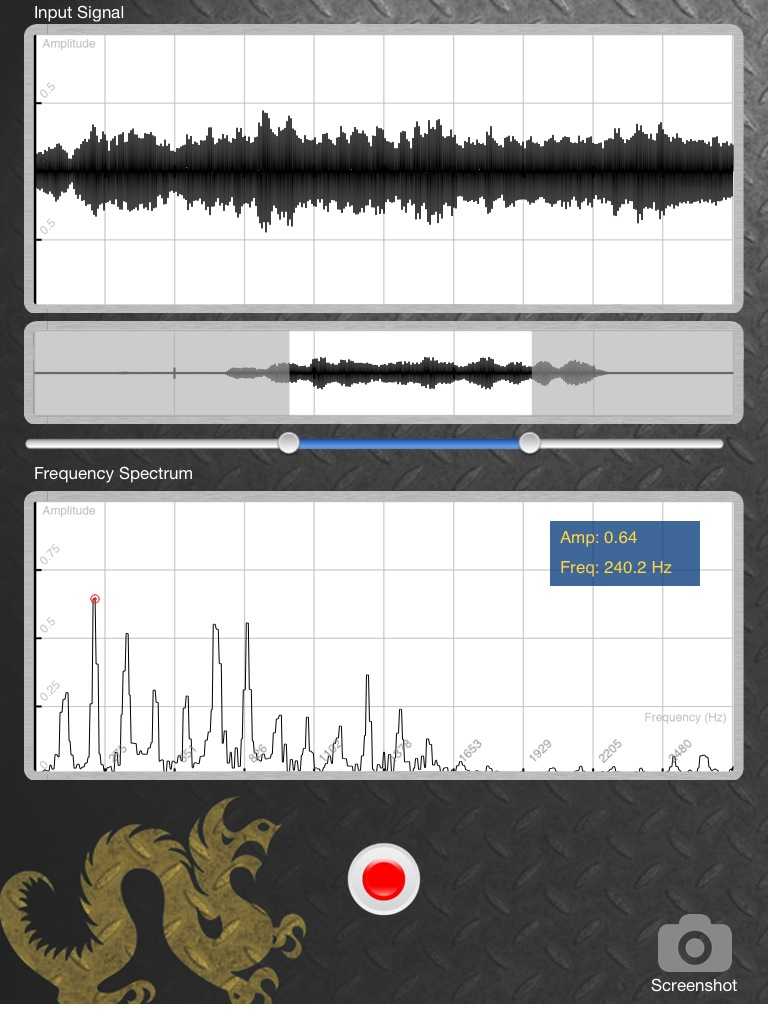
\includegraphics[width=4in]{images/Screenshots/SoundAnalysisApp}
\caption{Recording application for the analyzer iPad, which displays recorded audio. The top window shows a short section of the recorded waveform, and the bottom window displays the corresponding frequency spectrum. The middle window displays the entire 5-second recording. The two slider points determine the time window shown in the top and middle windows.}
\label{analyzerProgram}
\end{figure}

\item Look at the plot of the frequency spectrum and determine the frequency of the peak shown in the window. You should notice that the measured frequency should be reasonably close to the value indicated under the frequency slider.
\end{enumerate}

Now we'll repeat this experiment, but record the audio coming out of the tube with the Microphone.
\begin{enumerate}
\item Position the mic just inside the end of the tube.
\item Open the \textbf{SoundAnalysis} program on the \textbf{Analyzer} iPad and press the record button. 
\item Look at the frequency spectrum (bottom window) and find the frequency of the largest peak. If performed correctly, this should approximate the frequency you specified on the \textbf{Synthesizer} iPad.
\item The measured signal in the Spectrum Window consists of multiple peaks unlike the previous example. These peaks are due to distortion from the amp, tube, and the speaker.
\item Repeat Step 2, except now select the Noise box for your input signal.
\end{enumerate}

\vspace{20pt}
\textbf{Question:} What do you notice about the Spectrum when noise is applied? What frequency (or frequencies) are observed in the noise?
\vspace{50pt}

\newpage

\section {Acoustic Resonance}
\subsection {Overview}
In this section we'll investigate \textbf{\emph{resonance}}, which is an important feature of musical instruments. Resonance is a key factor in determining the way an instrument sounds (also known as its \emph{timbre}) as well as the frequency(s) an acoustic body will emphasize. In general physics, resonance is the tendency of a mechanical system (i.e. a pipe or suspension bridge) to absorb more energy when it is driven by its natural frequency(s).

\subsection{Experimentally Determining the Resonance Frequency}
\begin{enumerate} 
\item Place the smaller diameter tube in the larger one so that the total length is 90 cm. Maintain this length through the experiment. 
\item Position the mic at the end of the tube and prop it  up so that it is not touching the walls of the tube.
\item Set the \textbf{Synthesizer} iPad to half volume.
\item Turn the amp on and set the Volume knob to the 12 o'clock position.
\item Select Sine Wave in the synthesizer program to generate a tone, setting the frequency using the frequency slider. For more accurate control of the slider, slide your finger upwards on the iPad, then move to the left and right to move the slider.
\item On the \textbf{Analyzer} iPad, press record to capture live microphone audio. 
\item Begin slowly moving the frequency slider. When you've found the resonance frequency, you should notice the tube vibrating stronger at that frequency than it does at others. In the Spectrum Window, you should notice that the peaks have a stronger amplitude than they do at nearby frequencies.
\item Record the observed resonant frequency in Table \ref{ResFreqTable}. Repeat the result for the other tube lengths listed in Table \ref{ResFreqTable}.
\end {enumerate}

\begin{table}[!h]
	\begin{center}
    		\begin{tabular}{| c | c |}
		    \hline
	    Length (cm) & Frequency (Hz) \\ \hline
	    90 & \\ \hline
	    100 & \\ \hline
	    110 & \\ \hline
	    120 & \\ \hline
	    \end{tabular}
	\caption{\label{ResFreqTable}Resonant frequencies for different tube lengths}
	\end{center}
\end{table}

\textbf{Question}: What is the relationship between the tube length and its calculated resonance frequency?

\newpage

\subsection{Standing Waves and Resonance}
\begin{wrapfigure}{r}{0.4 \textwidth}
	\vspace{-20pt}
	\begin{center}
	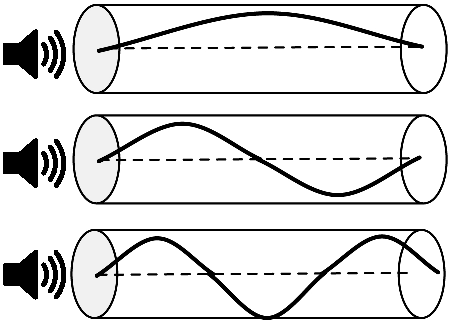
\includegraphics[width= .35 \textwidth]{images/resonance/harmonics2.pdf}
	\vspace{-10pt}
	\caption{\label{tubeResonances}Pressure signals from different tones forming standing waves in a tube.}
	\end{center}
	\vspace{-10pt}
\end{wrapfigure}

You probably noticed that there is in fact an \emph{inverse} relationship between the tube length and resonance frequency. That is, when the length of the tube is increased, the resonance frequency decreases and vice versa. To better understand why this occurs, we must take a closer look at what is occurring in the tube.

When the speaker is driven by a tone, a pressure signal from the speaker is applied to the tube. At resonance frequencies, the pressure signal is reflected at the end of the tube and adds together with the original to form a \emph{standing wave}. Standing waves arising from various resonance frequencies are shown in Figure \ref{tubeResonances}. Notice that the pressure is minimum at the tube's ends, so that any wave shape that ``fits'' the tube this way will produce a resonance.

But how do we calculate these resonant frequencies? Recall that the \emph{wavelength} of a sound wave describes the distance between two repeating points in the wave. Figure \ref{tubeResonances} shows that the resonant frequencies have a wavelength that is an integer number multiplied by $\lambda/2$, where $\lambda$ represents the wavelength. All of this means that:
\begin{enumerate}
\item \textbf{Acoustic tubes have many resonance frequencies}
\item \textbf{If we know the tube's dimensions, we can calculate the resonance frequencies}
\end{enumerate}

\begin{equation}
f = \frac{nv}{2 \left (L + .8d \right)}
\label{resonanceEq}
\end {equation}

Equation \ref{resonanceEq} shows how to compute the resonance frequencies for a tube with open ends (i.e. air can move freely in and out of both ends of the tube). The variable $n$ indicates the resonance index, or \emph{harmonic} number, $v$ is the speed of sound (340 meters/sec), and $L$ and $d$ are the tube's length and diameter in meters, respectively.

\vspace{15pt}

\textbf{Question}: Use Equation \ref{resonanceEq} to calculate the first 3 resonance frequencies for a 90 cm long open tube. Experimentally verify these frequencies using the analyzer program. Are the calculated resonances similar to the ones you observed? Record your results in Table \ref{EstResFreqTable}. (Hint: average the two different diameters of the two tubes for $d$. Convert centimeters to meters!!)

\begin{table}[h]
	\begin{center}
    		\begin{tabular}{| c | c | c |}
		    \hline
	    Resonant Frequency ($n$) & Theoretical (Hz) & Observed (Hz) \\ \hline
	    1 & &\\ \hline
	    2 & &\\ \hline
	    3 & &\\ \hline
	    \end{tabular}
	\caption{\label{EstResFreqTable} Theoretical and observed resonant frequencies for a 90 cm length tube}
	\end{center}
\end{table}

\vspace{.4in}

\textbf{Question}: Which resonant frequencies appear to be the strongest? The fundamental (i.e. $n = 1$) or the harmonically related resonances ($n=2, 3$). Analyze the amplitudes using the \textbf{Spectrum} Window to justify your answer.
\vspace{.5in}

\subsection{Filtering Noise with the Tube}
In the previous experiments, we have shown that we can estimate the resonant frequencies if we know the dimensions of the tube or the test frequencies used to drive it. However, if this information is unknown, we can try a different method. Recall that a noise signal contains energy at all frequencies. Since we know that tubes ``selectively'' resonate at certain frequencies, it may be easier to identify resonances by driving a tube with a signal that contains all frequencies.

\begin{enumerate}
\item Configure the tubes so that the total length is 90 cm.
\item Using the \textbf{Synthesizer} iPad, select Noise output and adjust the volume appropriately.
\item Observe the Spectrum on the \textbf{Synthesizer} iPad
\item On the \textbf{Analyzer} iPad, press record to analyze the tube audio
\item Observe the Spectrum on the \textbf{Analyzer} iPad and compare to the \textbf{Synthesizer}.
\end{enumerate}

\textbf{Question}: Compare and contrast the Spectrum Windows on the Analyzer and Synthesizer iPads. How are they different, if at all, and why?
\vspace{1.2in}


\textbf{Question}: Describe how you can identify the resonance frequencies when a noise signal is applied? Are the resonance frequencies you observe close to the ones you obtained using the previous methods?
\vspace{.6in}

\end{document}
